\documentclass{article}

\usepackage{graphicx}
\usepackage[utf8x]{inputenc}
\usepackage{url}
\usepackage{acronym}
\usepackage{tikz}
\usepackage{bm}
\usepackage{subcaption}
\usepackage[section]{placeins}
\usetikzlibrary{calc,positioning,shapes,decorations.pathreplacing}

\tikzset{
short/.style={draw,rectangle,text height=3pt,text depth=13pt,
  text width=7pt,align=center,fill=gray!30},
long/.style={short,text width=1cm},
double/.style={short,text width=2cm}
}



\begin{document}
% the long nodes \lnode{<label>}{<right of>}
\def\snode#1#2#3{%
  \node[long,right=of #1, label=center:#3] (#2) {}}

\def\dnode#1#2#3{%
  \node[double,right=of #1, label=center:#3] (#2) {}}


\begin{titlepage}
	\begin{center}
   	{\scshape\LARGE
    	Department of Information Engineering and Computer Science\\
      	(DISI)\\
      	University of Trento, Italy\\\par}
      	\vspace{1cm}
      	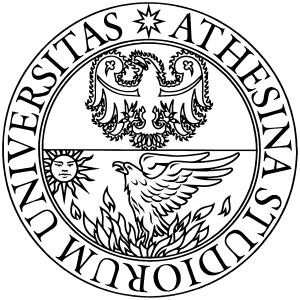
\includegraphics[scale=0.35]{logo}\\
	\vspace{1cm}
	{\scshape\Large Network Security - AY 2017/2018 \par}
	\vspace{1cm}
	{\huge\bfseries Lab Activity Report\\\par}
	\noindent\makebox[\linewidth]{\rule{\linewidth}{0.4pt}}
	{\Large\bfseries Man in the Middle attacks\par}
      	\noindent\makebox[\linewidth]{\rule{\linewidth}{0.4pt}}

        \vspace{.5cm}
        Author: \\
       	Gabriele Gemmi [198042] \\
				Lorenzo Brugnera [197054]
      	\vfill
      	\vfill
	\end{center}
\end{titlepage}

\section{Introduction}
\acrodef{MitM}{Man in the Middle}
\paragraph{What are \ac{MitM} attacks}
\begin{figure}[h]
\center
\includegraphics[width=.8\textwidth]{../figures/mitm_diagram}
\caption{Diagram of a MitM attack}
\end{figure}
\subsection{Network attacks}
\subsection{Service attacks}
\subsubsection{ARP Poisoning}
\begin{figure}[h]
  \center
  \includegraphics[width=.8\textwidth]{../figures/arp_spoofing}
  \caption{ARP Spoofing attack diagram}
\end{figure}
\paragraph{Countermeasures}
\subsubsection{DHCP Poisoning}
\begin{figure}[h]
\center
\includegraphics[width=.8\textwidth]{../figures/dhcp_poisong}
\caption{DHCP poisoning attack diagram}
\end{figure}

\paragraph{Countermeasures}
\begin{figure}[h]
\center
\includegraphics[width=.8\textwidth]{../figures/dhcp_snooping}
\caption{DHCP snooping diagram}
\end{figure}

\subsubsection{Evil Twin}
\begin{figure}[h]
  \center
  \includegraphics[width=.8\textwidth]{../figures/evil-twin}
  \caption{Evil Twin attack diagram}
\end{figure}
\paragraph{Countermeasures}
\section{Laboratory activity overview}
\begin{figure}[h]
  \center
  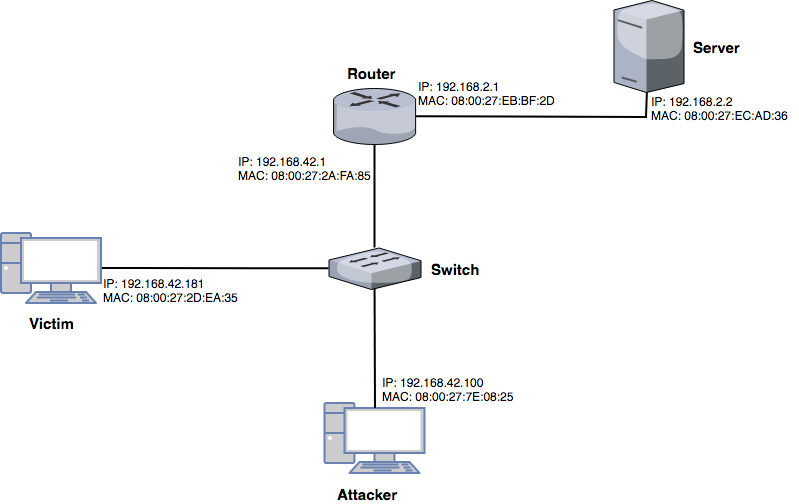
\includegraphics[width=.8\textwidth]{../figures/net_topo}
  \caption{Topology of the VMs network}
\end{figure}
\section{Exercises}
\subsection{Exercise 1 - SSL Stripping}
\begin{figure}[h]
  \center
  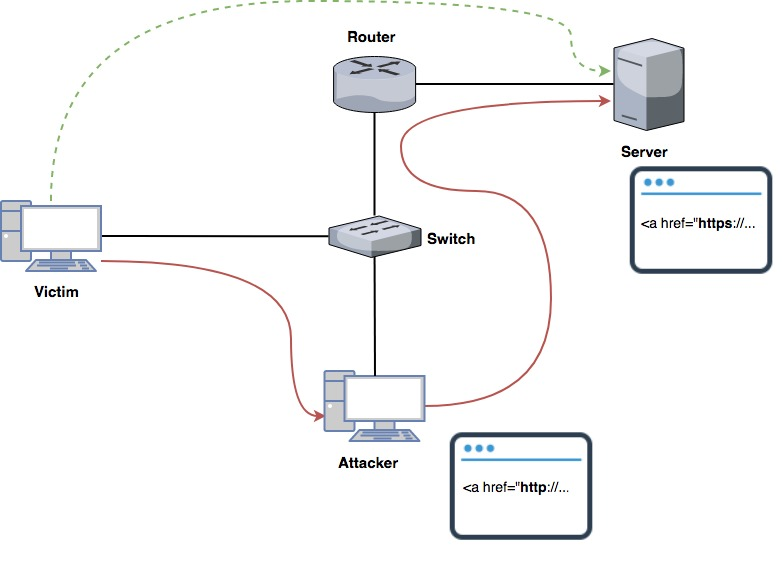
\includegraphics[width=.8\textwidth]{../figures/sslstrip}
  \caption{SSL Stripping attack diagram}
\end{figure}
\begin{figure}[h]
  \center
  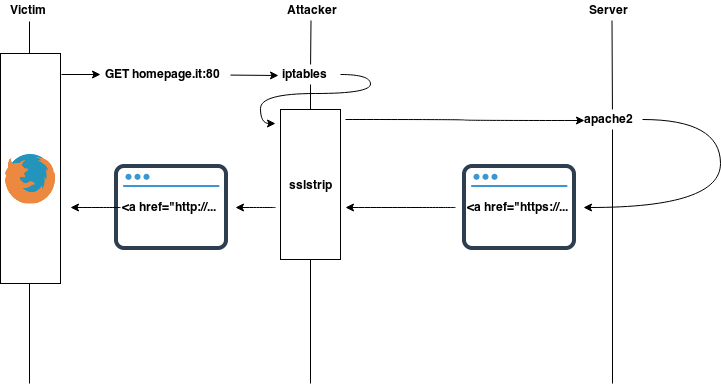
\includegraphics[width=.8\textwidth]{../figures/sslstrip_time}
  \caption{SSL Stripping attack diagram}
\end{figure}
% \begin{figure}
%   \center
%   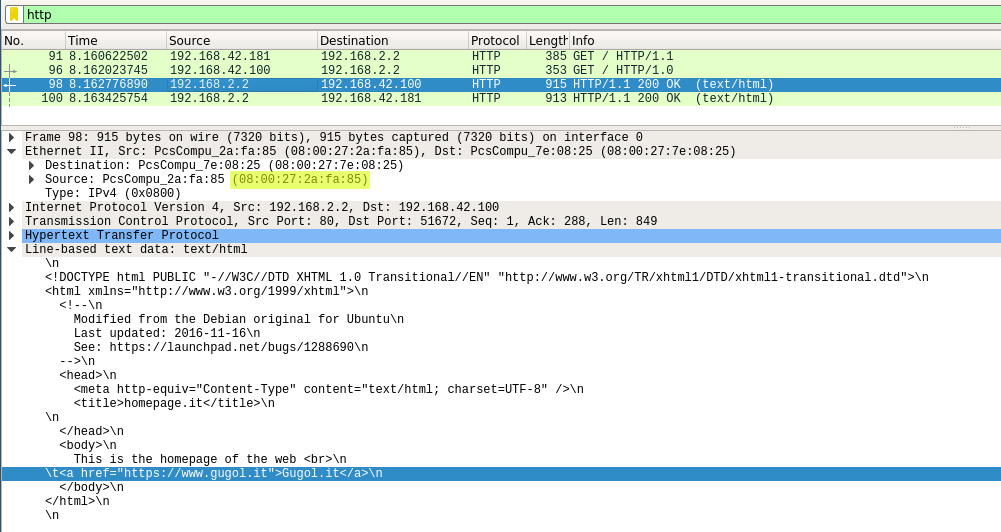
\includegraphics[width=\textwidth]{../figures/sslstrip_https}
%   \caption{}
% \end{figure}

\subsection{Exercise 2 - HSTS Bypassing}
\begin{figure}[h]
  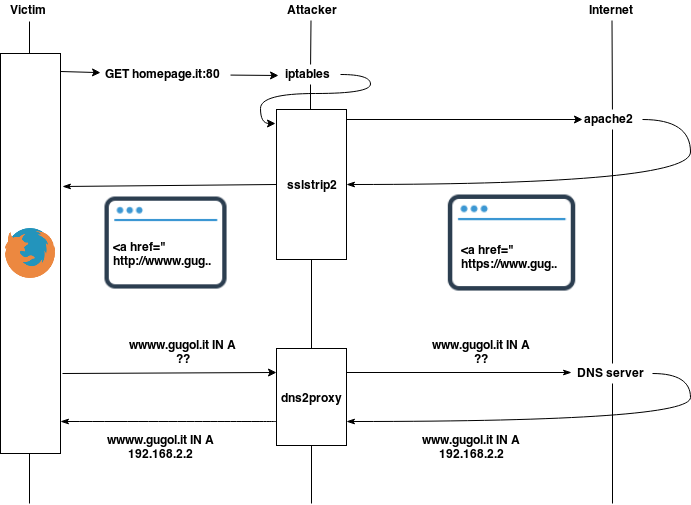
\includegraphics[width=.9\textwidth]{../figures/hsts_bypass_time}
  \caption{}
\end{figure}

\end{document}
